\documentclass[tikz,border=8pt]{standalone}
% Shared look for every TikZ diagram. Load with \input{../../tools/tikz-style.tex}
\usepackage[sfdefault]{roboto}
\usetikzlibrary{arrows.meta, positioning, shapes.geometric, calc, fit, backgrounds}
\definecolor{cblue}{HTML}{4C78A8}
\definecolor{corange}{HTML}{F58518}
\definecolor{cgreen}{HTML}{54A24B}
\definecolor{cred}{HTML}{E45756}
\definecolor{cpurple}{HTML}{B279A2}
\definecolor{cgrey}{HTML}{6B6B6B}
\tikzset{
  every picture/.style={font=\sffamily, line width=1.2pt},
  box/.style={draw=#1, fill=#1!12, rounded corners=4pt, align=center, inner sep=7pt, minimum height=1.1cm},
  box/.default=cgrey,
  arrow/.style={-{Stealth[length=3mm]}, draw=cgrey, line width=1.4pt},
  title/.style={font=\sffamily\bfseries\Large},
  note/.style={font=\sffamily\small, text=cgrey, align=center},
}
\AtBeginDocument{\hyphenpenalty=10000 \exhyphenpenalty=10000}

% One optimisation, two loops. Refine once: a search or sampling planner's path is the first guess (Apollo's
% open-space planner: Hybrid A* then smoothing; MoveIt: OMPL then CHOMP or STOMP), a controller then tracks the
% result. Re-plan every cycle: the last plan, shifted, is the first guess of the next solve (TEB, Autoware, Apollo on
% public roads).
\begin{document}
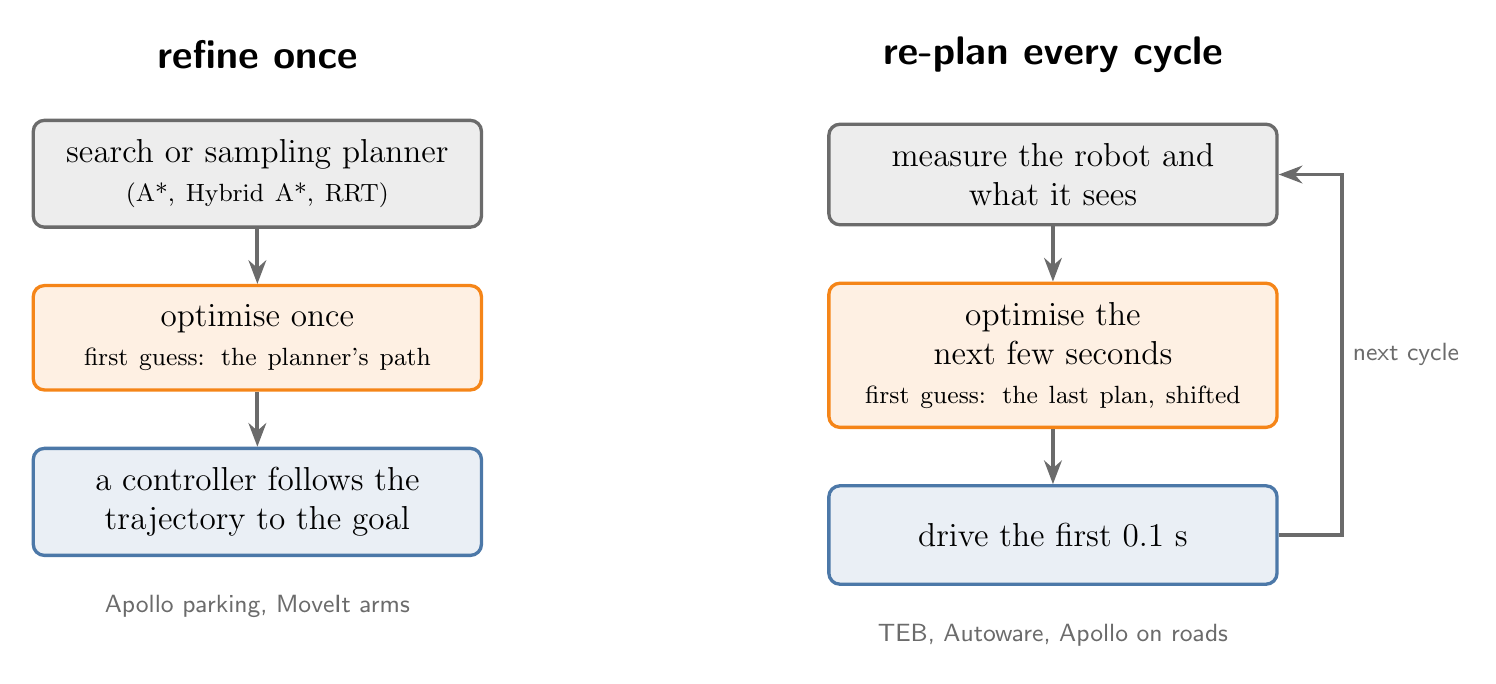
\begin{tikzpicture}[every node/.append style={font=\large}, node distance=0.7cm,
  st/.style={box=#1, minimum width=5.6cm, text width=5.2cm, minimum height=1.25cm}]
  % refine once
  \node[title] (t1) {refine once};
  \node[st=cgrey, below=0.5cm of t1] (a1) {search or sampling planner\\ \small (A*, Hybrid A*, RRT)};
  \node[st=corange, below=of a1] (a2) {optimise once\\ \small first guess: the planner's path};
  \node[st=cblue, below=of a2] (a3) {a controller follows the\\ trajectory to the goal};
  \draw[arrow] (a1) -- (a2); \draw[arrow] (a2) -- (a3);
  \node[note, below=0.35cm of a3, text width=5.6cm] {Apollo parking, MoveIt arms};
  % re-plan every cycle
  \node[title, right=6.4cm of t1] (t2) {re-plan every cycle};
  \node[st=cgrey, below=0.5cm of t2] (b1) {measure the robot and\\ what it sees};
  \node[st=corange, below=of b1] (b2) {optimise the next few seconds\\ \small first guess: the last plan, shifted};
  \node[st=cblue, below=of b2] (b3) {drive the first 0.1 s};
  \draw[arrow] (b1) -- (b2); \draw[arrow] (b2) -- (b3);
  \draw[arrow] (b3.east) -- ++(0.8,0) |- node[note, pos=0.25, right] {next cycle} (b1.east);
  \node[note, below=0.35cm of b3, text width=5.6cm] {TEB, Autoware, Apollo on roads};
\end{tikzpicture}
\end{document}
